% ============================================================================
% DeepREAP: Integrating Regressive Ensemble Demand Prediction with Deep
% Reinforcement Learning for Cloud Resource Allocation
%
% Version targeting ~10-11 pages (LNNS / svproc-compatible).
% Document class: llncs (also valid for LNNS submissions).
% References typed inline in splncs04 style.
% ============================================================================

\documentclass[runningheads]{llncs}

\usepackage[T1]{fontenc}
\usepackage{graphicx}
\usepackage{booktabs}
\usepackage{multirow}
\usepackage{amsmath}
\usepackage{amssymb}
\usepackage{microtype}
\usepackage{tikz}
\usetikzlibrary{positioning,arrows.meta,shapes.geometric,fit,calc}
\usepackage{xcolor}
\usepackage[hidelinks]{hyperref}
\usepackage{cleveref}

% ---------- Custom commands -------------------------------------------------
\newcommand{\reap}{\textsc{Reap}}
\newcommand{\deeprm}{\textsc{DeepRM\_Plus}}
\newcommand{\deepreap}{\textsc{DeepReap}}
\newcommand{\sjf}{\textsc{Sjf}}

\begin{document}

% ---------- Title / Authors -------------------------------------------------
\title{DeepREAP: Integrating Regressive Ensemble Demand Prediction with Deep Reinforcement Learning for Cloud Resource Allocation}
\titlerunning{DeepREAP: Demand Prediction Meets Deep RL Scheduling}

\author{Suma Nagral\inst{1} \and Raghav Sharma\inst{1}}
\authorrunning{S.~Nagral and R.~Sharma}

\institute{Department of Computer Engineering, San Jose State University,
San Jose, CA, USA\\
\email{\{suma.nagral,raghav.sharma\}@sjsu.edu}}

\maketitle

% ---------- Abstract --------------------------------------------------------
\begin{abstract}
Cloud resource allocation is complicated by the dynamic and
heterogeneous nature of cloud workloads, and small and medium
enterprises (SMEs) disproportionately absorb the resulting
inefficiency. Prior work advances along two largely independent axes:
deep reinforcement learning (DRL) schedulers such as \deeprm{}, which
react to the current cluster state, and regression ensembles such as
the Regressive Ensemble Approach for Prediction (\reap{}), which
forecast future demand. We present \deepreap{}, which couples the two
by fusing \reap{}'s demand forecast directly into the state
representation of a convolutional DRL scheduler, realising as working
software an architecture previously specified only conceptually. On a
60-day synthetic trace the \reap{} ensemble attains MSE $8.07$ on the
CPU-load target, improving on every constituent regressor. On a shared
$3{,}000$-job trace the \deepreap{} imitation policy reduces average
job slowdown to $8.27$ against $20.11$ for shortest-job-first and
$18.76$ for a Tetris-style packer --- a $2.4\times$ improvement --- and
lowers average completion time from $49.51$ to $19.04$ slots. Isolating
the forecast channels as the only difference from \deeprm{} attributes
the gain to prediction rather than architecture. We report the costs
alongside: the policy completes fewer jobs under a fixed step budget,
PPO refinement degrades rather than improves the imitation checkpoint
at the training budget available, and the ensemble does not dominate
its base models on the memory target. Code, seeds, and per-run outputs
are released to support replication.
\keywords{Cloud resource allocation \and Deep reinforcement learning
\and Ensemble regression \and Job scheduling \and Demand prediction
\and Imitation learning}
\end{abstract}

% ============================================================================
\section{Introduction}
% ============================================================================
Cloud resource allocation --- distributing compute, memory, and network
capacity across running applications --- determines service
performance, operational cost, and user experience. It is also hard,
because cloud environments are dynamic and the demands placed on them
heterogeneous. Small and medium enterprises (SMEs) feel this acutely:
they rarely employ dedicated capacity-planning staff and lack the scale
over which large providers amortise over-provisioning, so an allocation
policy that is merely adequate at hyperscale can be materially
expensive for an SME~\cite{osypanka2022}.

Two families of machine-learning techniques address this. DRL
schedulers learn an allocation policy from interaction with the
cluster; DeepRM~\cite{mao2016} and its successor
\deeprm{}~\cite{guo2021} are canonical. Separately, regression models
forecast future demand from historical telemetry, enabling
provisioning decisions before demand
materialises~\cite{bankole2013,kaur2019}. The two are complementary ---
one is reactive and optimises sequencing, the other anticipatory --- yet
they are seldom combined.

We frame the integration along a single axis: \emph{what the scheduler
knows about the future}. A vanilla DRL scheduler observes only the
current cluster state and the visible job queue, so its decisions are
myopic: it commits capacity to the job that looks best now, with no
signal about whether that capacity will be scarce or idle a few steps
later. A scheduler that additionally observes a forecast of demand over
its planning horizon can, in principle, act on that signal --- most
directly, it can defer a long job that would occupy a resource through
an anticipated demand spike, and place it instead in a window the
forecast marks as idle. This is the mechanism we hypothesise will
reduce job slowdown, and it is the behaviour we later observe
(\cref{sec:sched-perf}). Crucially, the forecast helps only if it is
\emph{accurate} and if the policy can \emph{learn to use it}; a wrong
or ignored forecast can only add noise to the state. The hypothesis is
therefore not self-evidently true, and testing it --- quantifying what
the forecast is worth, and what it costs --- is the contribution, rather
than any new learning algorithm. We fuse the forecast into the state
representation rather than post-processing it into a priority score
precisely so that the policy, not the designer, decides how much to
trust it.

An earlier conceptual study proposed \deepreap{}, uniting the \reap{}
ensemble predictor~\cite{kaur2019} with the \deeprm{}
scheduler~\cite{guo2021}. That study was explicitly limited to a plan
and a theoretical framework: it conducted no implementation, testing,
or validation, and stated that the system's real-world viability
remained speculative. The present paper closes that gap.

\textbf{Contributions.}
(i)~A working \deepreap{} implementation --- \reap{} prediction, DRL
scheduling, a REST integration layer, and a Prometheus/Grafana
monitoring loop --- as runnable software rather than a specification.
(ii)~A concrete state-fusion mechanism injecting a demand forecast into
the scheduler's state as additional image channels, requiring no change
to the policy architecture and no hand-coded contract between predictor
and agent. (iii)~An empirical evaluation against three heuristic and
two DRL baselines on a shared trace, isolating the forecast as the
single independent variable: slowdown falls from $19.30$ to $8.27$ and
completion from $43.41$ to $19.04$ slots. (iv)~Honest scoping of the
negative results --- PPO refinement degrades both pre-trained policies
at our budget, the slowdown gain is paid for in throughput, and
inverse-MSE ensemble weighting is too flat to beat the strongest base
model on one of two targets. Code, fixed seeds, checkpoints, and raw
benchmark output are released for replication.

% ============================================================================
\section{Related Work}
% ============================================================================
\paragraph{Learning to schedule.} Early approaches allocate by
priority: Son and Buyya~\cite{son2019} combine priority-aware VM
allocation with bandwidth provisioning in SDN-enabled clouds, and
Savitha and Salvi~\cite{savitha2021} learn application priorities from
historical usage; both are validated in simulation and depend on the
consistency of historical data. Reinforcement learning removes the need
for hand-designed priority rules. Mao et al.~\cite{mao2016} introduced
DeepRM, formulating cluster scheduling over an image-like state
encoding and outperforming classical heuristics. Guo
et al.~\cite{guo2021} extended it into \deeprm{}, using imitation
learning to accelerate convergence and improving average weighted
turnaround time. Zhou et al.~\cite{zhou2021} pair a DRL agent with a
policy set enforcing SLA constraints. Recurring concerns across this
line are generalisability across platforms, scalability to larger
deployments, and the data appetite of training.

\paragraph{Learning to predict.} A parallel literature forecasts demand
rather than sequencing it. Bankole and Ajila~\cite{bankole2013} find
SVM strongest among classical regressors for provisioning prediction
($4.5\%$ average error), and show that including SLA metrics improves
accuracy further. Osypanka and Nawrocki~\cite{osypanka2022,osypanka2023}
report up to $85\%$ cost reduction from ARIMA-based and self-adapting
long-term predictors without QoS degradation. Gyeera
et al.~\cite{gyeera2023} reach $R^2=0.9991$ on data-centre KPI
forecasting with Boosted Decision Trees, at appreciable training cost.
Most relevant here, Kaur, Bala, and Chana~\cite{kaur2019} propose
\reap{}, which selects features by genetic algorithm, trains multiple
regressors on the selected subset, and combines them in an
accuracy-weighted ensemble, reaching $95\%$ accuracy on a real-world
dataset. Its costs are training expense and uncertain transferability
across cloud environments.

\paragraph{The gap.} DRL schedules well; regression ensembles predict
well. Their integration into a single framework --- in which
anticipated demand conditions the scheduling policy itself --- remains
underexplored, and is what we implement and evaluate.

% ============================================================================
\section{Methodology}\label{sec:methodology}
% ============================================================================
\Cref{fig:pipeline} overviews the architecture, which comprises four
modules connected by well-defined data interfaces.

\textbf{(1) Demand prediction (\reap{}).} \emph{Input:} a row of
resource telemetry --- timestamp, service type, active users, previous
hour's CPU, network utilisation. \emph{Output:} a scalar demand
prediction per target (CPU load, memory usage). Internally it selects
features by genetic algorithm and combines five regressors into an
accuracy-weighted ensemble (\cref{sec:reap}).

\textbf{(2) Resource scheduling (\deeprm{}).} \emph{Input:} a
multi-channel state image encoding cluster occupancy and the visible
job queue. \emph{Output:} a scheduling action --- schedule a visible
job or no-op. Internally a CNN policy, pre-trained by imitation of a
\sjf{} expert and refined with PPO, maps state to action
(\cref{sec:training}).

\textbf{(3) State fusion (the integration point).} This module rolls
\reap{} forward over the scheduler's planning horizon and appends the
forecast to the state image as extra channels, so modules~(1) and~(2)
communicate through the state tensor itself rather than a bespoke
protocol (\cref{sec:env}). It is the sole structural difference between
\deepreap{} and a vanilla \deeprm{} scheduler.

\textbf{(4) Serving and monitoring.} A FastAPI service exposes
\texttt{/predict}, \texttt{/forecast}, \texttt{/schedule}, and
\texttt{/feedback} endpoints; Prometheus scrapes \texttt{/metrics} and
Grafana visualises them. Observed values posted to \texttt{/feedback}
update a prediction-error gauge, giving the operator a live view of
whether the forecast the scheduler consumes is tracking reality.

The critical design choice is in module~(3): forecasts are \emph{fused
into the state} rather than post-processed into a priority score, so
the policy learns for itself how much to trust them.

\begin{figure}[t]
\centering
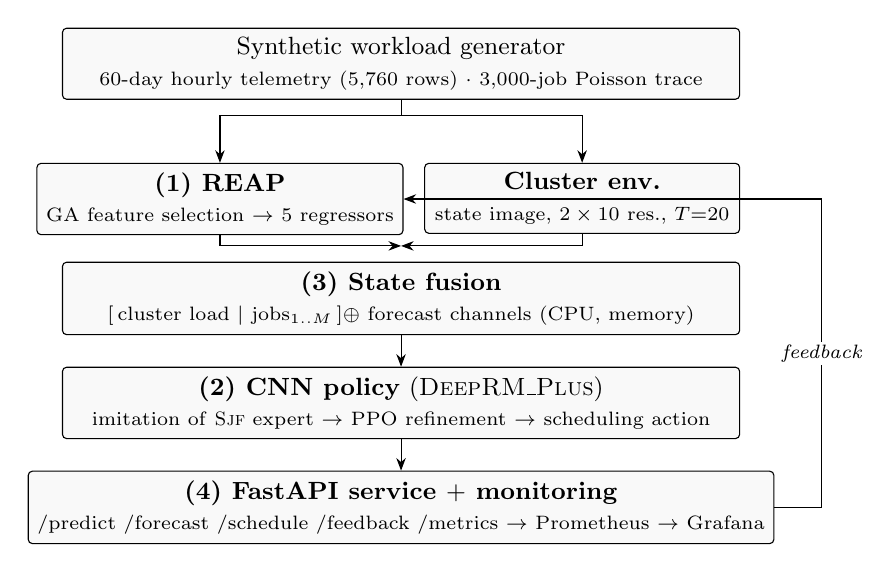
\begin{tikzpicture}[
  font=\small,
  node distance=4mm and 4mm,
  box/.style={draw, rounded corners=1.5pt, align=center, minimum width=8.6cm,
              minimum height=8mm, fill=gray!5},
  smallbox/.style={draw, rounded corners=1.5pt, align=center,
                   minimum width=4.0cm, minimum height=8mm, fill=gray!5},
  arr/.style={-{Stealth[length=1.6mm]}}
]
\node[box] (gen) {Synthetic workload generator\\ \scriptsize 60-day hourly telemetry (5{,}760 rows) $\cdot$ 3{,}000-job Poisson trace};
\node[smallbox, below=8mm of gen, xshift=-2.3cm] (reap) {\textbf{(1) REAP}\\\scriptsize GA feature selection $\to$ 5 regressors};
\node[smallbox, below=8mm of gen, xshift=2.3cm] (env) {\textbf{Cluster env.}\\\scriptsize state image, $2\times10$ res., $T{=}20$};
\node[box, below=8mm of $(reap)!0.5!(env)$] (fuse) {\textbf{(3) State fusion}\\ \scriptsize $[\,$cluster load $\mid$ jobs$_{1..M}\,] \oplus$ forecast channels (CPU, memory)};
\node[box, below=of fuse] (pol) {\textbf{(2) CNN policy} (\deeprm{})\\ \scriptsize imitation of \textsc{Sjf} expert $\to$ PPO refinement $\to$ scheduling action};
\node[box, below=of pol] (api) {\textbf{(4) FastAPI service $+$ monitoring}\\ \scriptsize /predict /forecast /schedule /feedback /metrics $\to$ Prometheus $\to$ Grafana};
\draw[arr] (gen.south) -- ++(0,-2mm) -| (reap.north);
\draw[arr] (gen.south) -- ++(0,-2mm) -| (env.north);
\draw[arr] (reap.south) |- ($(fuse.north)+(0,2mm)$);
\draw[arr] (env.south)  |- ($(fuse.north)+(0,2mm)$);
\draw[arr] (fuse) -- (pol);
\draw[arr] (pol) -- (api);
\draw[arr] (api.east) -- ++(6mm,0) |- node[font=\scriptsize\itshape,
  fill=white, inner sep=1pt, pos=0.25] {feedback} (reap.east);
\end{tikzpicture}
\caption{The \deepreap{} pipeline. Numbered boxes correspond to the
four modules described in \cref{sec:methodology}; numbers follow the
module roles in the text rather than top-to-bottom dataflow, so state
fusion~(3) precedes the scheduling policy~(2) it feeds. \reap{}
forecasts~(1) and the raw cluster state are fused into a single
multi-channel state image before reaching the policy, so no hand-coded
contract binds predictor to agent. The feedback path updates a
prediction-error gauge; \reap{} weights themselves are frozen after
fitting (see \cref{sec:limitations}).}
\label{fig:pipeline}
\end{figure}

\subsection{Workload Generation}\label{sec:data}
The original proposal assumed historical resource usage without
specifying a trace, so we generate one with realistic structure.
\textbf{Resource usage:} hourly records for four service types (Web,
Database, Media, Compute) with diurnal and weekly cycles, an
autoregressive dependence on the previous hour's CPU, and Gaussian
noise --- $60$ days $\times\,4$ services $=5{,}760$ rows.
\textbf{Job trace:} Poisson arrivals; bimodal durations ($80\%$ short
jobs of $1$--$3$ slots, $20\%$ long jobs of $10$--$15$ slots); bimodal
per-resource demand with one dominant resource per job, matching the
regime of Mao et al.~\cite{mao2016} --- $3{,}000$ jobs over $1{,}500$
timesteps. Seeds are fixed throughout (data $42/43$, \reap{} $42$,
DeepRM $42$, benchmark $123$).

\subsection{REAP Demand Prediction}\label{sec:reap}
\textbf{Feature selection.} A chromosome is a binary mask over
candidate features, with fitness
$-\mathrm{CV\_MSE}-0.01\cdot|\text{features}|$ for a Ridge regressor on
the selected subset ($3$-fold CV, $25$ generations, population $24$,
tournament-$3$ selection, single-point crossover, $5\%$ mutation).
\textbf{Base regressors.} Linear Regression, Bayesian Ridge, Decision
Tree, Random Forest, and SVR (RBF) --- the families named in the \reap{}
formulation~\cite{kaur2019} --- are each trained on the selected feature
subset over the training split.

\textbf{Ensemble.} The five fitted regressors are combined in three
steps. First, each model $m$ is scored on a held-out validation split,
yielding a mean squared error $\mathrm{MSE}_m$. Second, each model is
assigned a weight inversely proportional to that error and the weights
are normalised to a convex combination,
\begin{equation}
w_m \;=\; \frac{1/\mathrm{MSE}_m}{\sum_{j=1}^{5} 1/\mathrm{MSE}_j},
\qquad \sum_{m=1}^{5} w_m = 1,
\label{eq:weights}
\end{equation}
so that a more accurate model contributes more to the final estimate.
Third, at inference the ensemble prediction for an input $\mathbf{x}$
is the weighted sum of the base predictions,
$\hat{y}(\mathbf{x}) = \sum_{m=1}^{5} w_m\, f_m(\mathbf{x})$, where
$f_m$ is the $m$-th fitted regressor. Weighting by inverse error rather
than training a meta-learner keeps the combiner parameter-free and
interpretable, but --- as \cref{sec:pred-perf} shows --- it is a weak
form of ensembling: when one base model is clearly strongest, the
$1/\mathrm{MSE}$ scaling does not concentrate enough weight on it to
beat that model alone.

\subsection{Scheduling Environment and State Fusion}\label{sec:env}
A discrete-time cluster scheduler with $2$ resources of capacity $10$
and horizon $T{=}20$; $M{=}5$ visible job slots plus a bounded backlog
of $60$. The state image is
$[\,\text{cluster load}\mid\text{job}_1\mid\dots\mid\text{job}_M\,]$
with shape $(1,R,T\cdot(M{+}1))$. Successful schedules do not advance
time, letting the agent fill several slots per timestep. The reward at
each time-advancing step is $-\sum_j 1/T_j$ over resident jobs, scaled
by $1/10$ for value-loss stability.

For \deepreap{}, \reap{} is rolled forward $T$ hours into a tensor of
shape $(C,R,T)$ appended as extra channels: channel~$0$ carries
predicted CPU demand broadcast across the resource axis and normalised
to $[0,1]$; channel~$1$ carries predicted memory demand under the same
convention. This is the \emph{only} difference between the \deeprm{}
and \deepreap{} configurations we compare, which is what licenses
attributing the performance difference to the forecast.

\subsection{Policy Network and Training}\label{sec:training}
The policy is two \texttt{Conv2d} blocks with $(1,3)$ kernels, an
\texttt{AdaptiveAvgPool2d} to $(1,16)$, and an MLP head emitting action
logits and a value estimate; the adaptive pool makes head size
independent of $T\cdot(M{+}1)$. \textbf{Imitation pre-training} runs an
\sjf{} expert for $30$ episodes ($\approx6{,}000$ transitions) and
trains the CNN by cross-entropy for $6$ epochs, reaching loss $0.53$ on
a $6$-class problem against a uniform-prior $\ln 6\approx1.79$.
\textbf{PPO refinement} uses a clipped objective with GAE
($\gamma{=}0.995$, $\lambda{=}0.95$, clip $0.1$, lr $10^{-4}$,
$4$~envs $\times\,256$-step rollouts, $3$ epochs/update,
$c_{vf}{=}0.25$, $c_{ent}{=}0.01$, grad-norm clip $0.5$) for $15$
updates. Both the imitation and post-PPO checkpoints are saved and
benchmarked separately.

\subsection{Evaluation Protocol}\label{sec:metrics}
All schedulers run on the \emph{same} job trace (seed $123$) for a
budget of $201$ environment steps. We report average slowdown (job
turnaround normalised by duration), average completion time in slots,
jobs completed $n_{\text{done}}$ within the budget, and total
environment reward. Baselines are three heuristics --- FIFO, \sjf{}, and
Packer (Tetris-style, selecting the visible job whose demand vector
maximises the dot product with free capacity) --- plus the imitation and
post-PPO checkpoints of both \deeprm{} and \deepreap{}. Prediction
quality is reported as MSE and MAE per base model and for the ensemble
on both targets.

% ============================================================================
\section{Results and Analysis}
% ============================================================================
We organise results around prediction accuracy
(\S\ref{sec:pred-perf}), scheduling performance
(\S\ref{sec:sched-perf}), and training dynamics
(\S\ref{sec:dynamics}).

\subsection{Prediction Accuracy}\label{sec:pred-perf}
\Cref{tab:reap} and \cref{fig:reap-quality} report per-model error on
both targets. On \texttt{cpu\_load} the ensemble improves on every
constituent regressor on both MSE and MAE, confirming that
accuracy-weighted combination is worthwhile. The genetic algorithm
selected $8$ of $11$ candidate features, discarding
\texttt{day\_of\_week}, \texttt{is\_weekend}, and
\texttt{svc\_Database} --- information already carried by
\texttt{hour\_of\_day}, the autoregressive term, and the remaining
one-hot indicators.

\begin{table}[!htbp]
\centering
\caption{\reap{} base-model and ensemble accuracy on both prediction
targets ($60$-day trace). Best per (target, metric) in bold. The
ensemble wins on \texttt{cpu\_load} but is beaten by SVR alone on
\texttt{memory\_usage}.}
\label{tab:reap}
\footnotesize
\setlength{\tabcolsep}{5pt}
\begin{tabular}{l l r r r}
\toprule
Target & Model & MSE & MAE & Weight \\
\midrule
\multirow{6}{*}{\texttt{cpu\_load}}
 & Linear Regression & 9.33  & 2.45 & 0.205 \\
 & Bayesian Ridge    & 9.34  & 2.45 & 0.205 \\
 & Decision Tree     & 14.47 & 2.99 & 0.132 \\
 & Random Forest     & 8.41  & 2.32 & 0.227 \\
 & SVR (RBF)         & 8.26  & 2.30 & 0.231 \\
 & \textbf{Ensemble} & \textbf{8.07} & \textbf{2.28} & --- \\
\midrule
\multirow{6}{*}{\texttt{memory\_usage}}
 & Linear Regression & 27.50 & 4.23 & 0.202 \\
 & Bayesian Ridge    & 27.50 & 4.23 & 0.202 \\
 & Decision Tree     & 34.68 & 4.69 & 0.160 \\
 & Random Forest     & 26.47 & 4.13 & 0.210 \\
 & \textbf{SVR (RBF)} & \textbf{24.49} & \textbf{4.00} & 0.227 \\
 & Ensemble          & 25.04 & 4.03 & --- \\
\bottomrule
\end{tabular}
\end{table}

\begin{figure}[!htbp]
\centering
\begin{minipage}{0.49\linewidth}
  \centering
  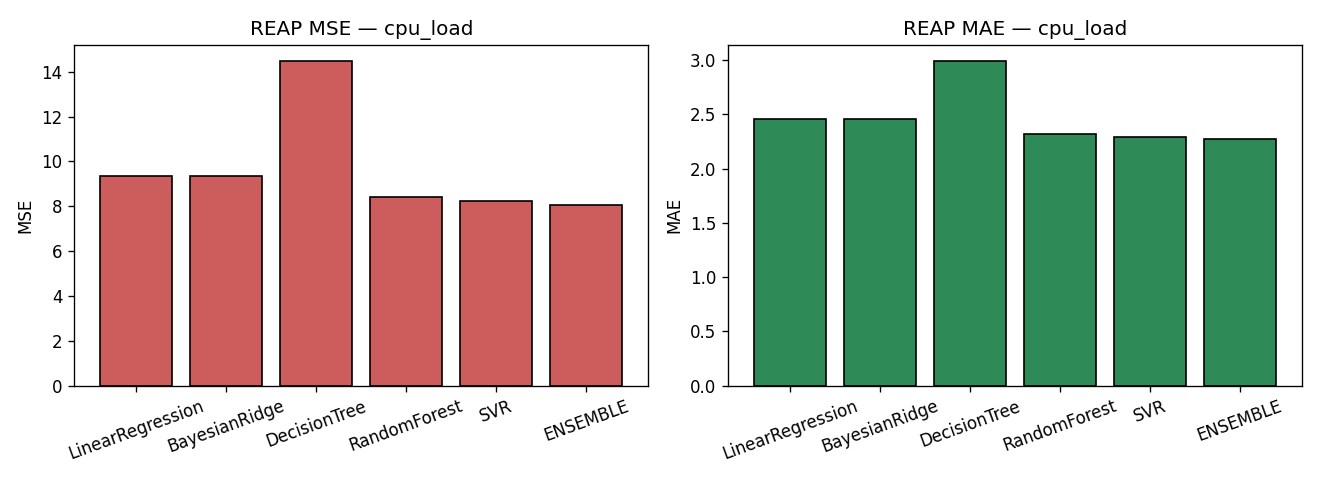
\includegraphics[width=\linewidth]{figures/reap_quality_cpu_load.png}
\end{minipage}\hfill
\begin{minipage}{0.49\linewidth}
  \centering
  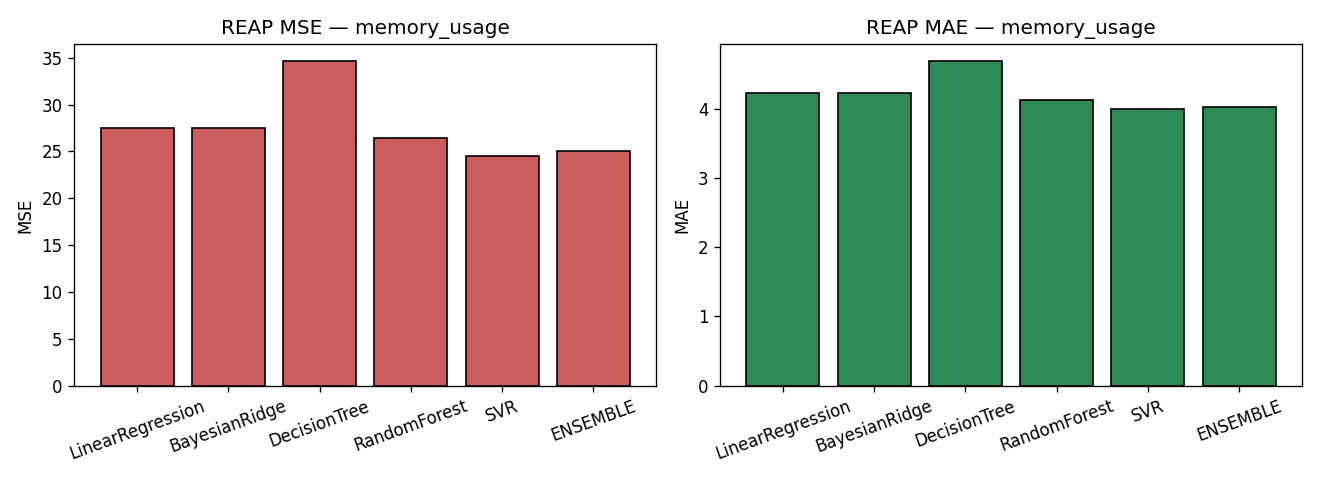
\includegraphics[width=\linewidth]{figures/reap_quality_memory_usage.png}
\end{minipage}
\caption{\reap{} base-model and ensemble error, MSE (left panel of
each pair) and MAE (right). \textbf{Left:} \texttt{cpu\_load} --- the
ensemble bar is lowest in both panels. \textbf{Right:}
\texttt{memory\_usage} --- the SVR bar edges below the ensemble,
illustrating the limits of inverse-MSE weighting.}
\label{fig:reap-quality}
\end{figure}

\paragraph{Where ensembling fails.} On \texttt{memory\_usage} the
ensemble (MSE $25.04$) does \emph{not} improve on its strongest
constituent, SVR ($24.49$). \Cref{fig:reap-weights} explains why:
inverse-MSE weighting is nearly flat, spanning only $0.13$--$0.23$
across both targets. The Decision Tree, at roughly $1.7\times$ the MSE
of SVR, is penalised far less than that ratio warrants, so the
ensemble is dragged toward weaker linear and tree models. The ensemble
still beats four of five base models and remains a reasonable default
when the best base model is not known in advance, but the claim that
ensembling dominates unconditionally is not supported by our data.
Sharper weighting --- softmax over $-\mathrm{MSE}$ with a temperature,
or top-$k$ selection --- would likely recover the gap.

\begin{figure}[!htbp]
\centering
\begin{minipage}{0.49\linewidth}
  \centering
  
\includegraphics[width=\linewidth]{figures/reap_weights_cpu_load.png}
\end{minipage}\hfill
\begin{minipage}{0.49\linewidth}
  \centering
  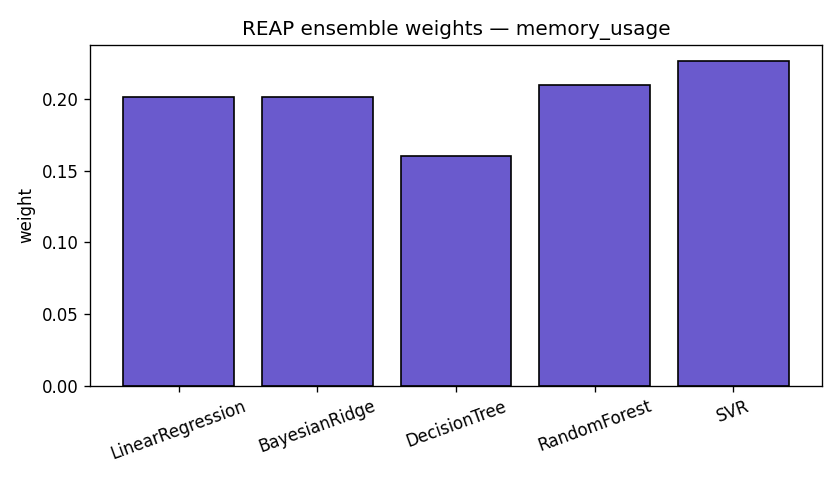
\includegraphics[width=\linewidth]{figures/reap_weights_memory_usage.png}
\end{minipage}
\caption{Accuracy-derived ensemble weights for \texttt{cpu\_load}
(left) and \texttt{memory\_usage} (right). Weights span only
$0.13$--$0.23$: inverse-MSE weighting approaches uniform when
base-model errors are of similar magnitude, which is the direct cause
of the memory-target result in \cref{tab:reap}.}
\label{fig:reap-weights}
\end{figure}

\subsection{Scheduling Performance}\label{sec:sched-perf}
\Cref{tab:bench} and \cref{fig:sched} report the scheduling benchmark.

\begin{table}[!htbp]
\centering
\caption{Scheduler comparison on a shared job trace (seed $123$,
$201$ steps). Arrows give the preferred direction; best per column in
bold. \deepreap{}'s imitation policy attains the best slowdown and
completion time and simultaneously the fewest completed jobs.}
\label{tab:bench}
\footnotesize
\setlength{\tabcolsep}{5pt}
\begin{tabular}{l r r r r}
\toprule
Scheduler & Slowdown $\downarrow$ & Completion $\downarrow$ &
$n_{\text{done}}$ $\uparrow$ & Reward $\uparrow$ \\
\midrule
FIFO   & 20.20 & 48.65 & \textbf{54} & $-374.6$ \\
\sjf{} & 20.11 & 49.51 & 53 & $\mathbf{-366.3}$ \\
Packer & 18.76 & 48.42 & 52 & $-375.3$ \\
\midrule
\deeprm{} (imitation) & 19.30 & 43.41 & 41 & $-414.1$ \\
\deeprm{} (PPO)       & 24.47 & 55.44 & 41 & $-443.7$ \\
\midrule
\textbf{\deepreap{} (imitation)} & \textbf{8.27} & \textbf{19.04} & 25 & $-446.4$ \\
\deepreap{} (PPO)     & 18.12 & 42.05 & 43 & $-401.8$ \\
\bottomrule
\end{tabular}
\end{table}

\begin{figure}[!htbp]
\centering
\begin{minipage}{0.49\linewidth}
  \centering
  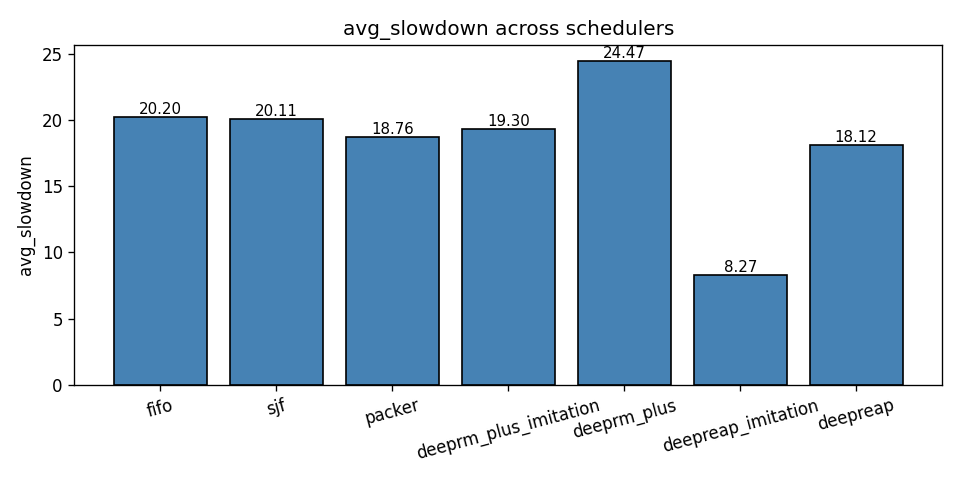
\includegraphics[width=\linewidth]{figures/avg_slowdown.png}
\end{minipage}\hfill
\begin{minipage}{0.49\linewidth}
  \centering
  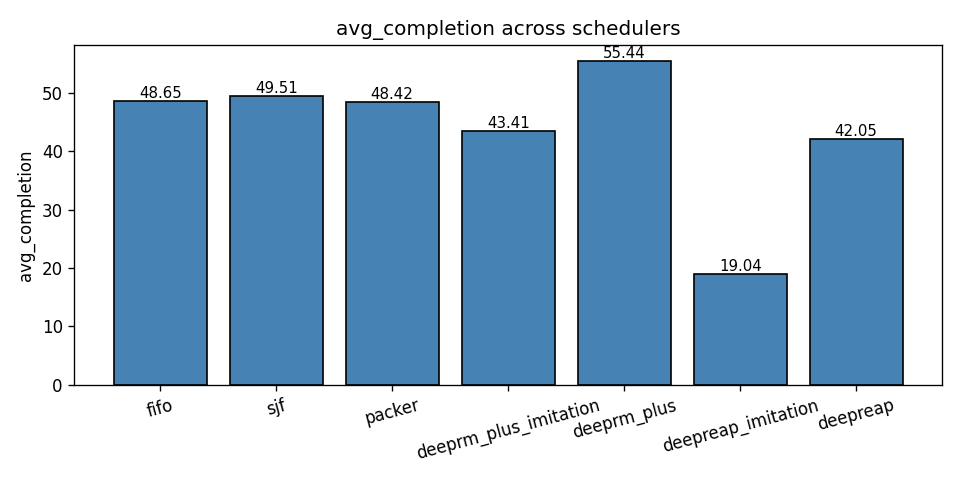
\includegraphics[width=\linewidth]{figures/avg_completion.png}
\end{minipage}
\caption{Average job slowdown (left) and average completion time in
slots (right) across all seven schedulers; lower is better in both.
\deepreap{}-imitation reaches $8.27$ slowdown, less than half the best
heuristic result of $18.76$, with the completion ordering closely
tracking it.}
\label{fig:sched}
\end{figure}

\paragraph{The forecast is what helps.} \deepreap{}-imitation achieves
average slowdown $8.27$ against $20.11$ for \sjf{} and $18.76$ for
Packer --- a $2.4\times$ improvement over the best baseline --- and cuts
average completion from $48.4$--$49.5$ slots to $19.04$. Because
\deepreap{} and \deeprm{} differ only in the forecast channels
(\cref{sec:env}) and share training procedure, seed, and evaluation
trace, the like-for-like comparison isolates the contribution: slowdown
$19.30\to8.27$, completion $43.41\to19.04$. The gain is attributable to
prediction, not to architecture or tuning.

\paragraph{And what it costs.} \deepreap{}-imitation completes $25$
jobs within the step budget against $52$--$54$ for the heuristics. The
policy learns to defer long jobs that would occupy capacity into
windows where \reap{} anticipates spare headroom, improving efficiency
on the jobs it does schedule while reducing raw throughput. Its total
reward ($-446.4$) is accordingly the worst in \cref{tab:bench}, because
the environment reward penalises every resident job at every step,
including those held in backlog. Slowdown and reward therefore measure
different things, and a deployment valuing throughput over per-job
latency would prefer the heuristics. We regard this as a genuine
limitation rather than a presentational detail: the improvement is real
but it is an improvement on a specific objective.

\subsection{Training Dynamics}\label{sec:dynamics}
\Cref{fig:curves} shows the PPO learning curves. Neither run converges:
mean episode reward oscillates between roughly $-400$ and $-200$ across
all $15$ updates with no downward trend in variance, and the two curves
are near-superimposable, both runs sharing seed $42$ and the forecast
channels apparently exerting little influence on PPO dynamics at this
budget. Refinement moved \deepreap{} slowdown from $8.27$ to $18.12$,
substantially overwriting what imitation had learned, and \deeprm{}
from $19.30$ to $24.47$ --- worse than every heuristic.

\begin{figure}[!htbp]
\centering
\begin{minipage}{0.49\linewidth}
  \centering
  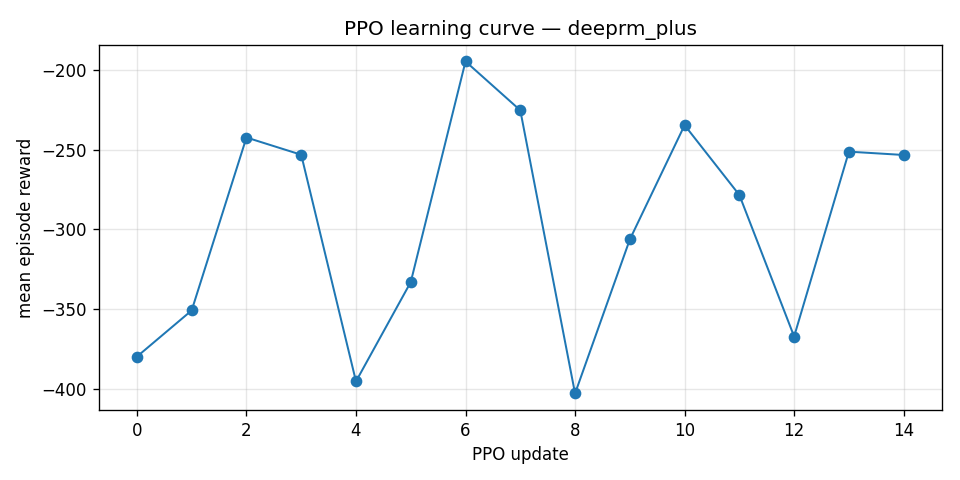
\includegraphics[width=\linewidth]{figures/learning_curve_deeprm_plus.png}
\end{minipage}\hfill
\begin{minipage}{0.49\linewidth}
  \centering
  
\includegraphics[width=\linewidth]{figures/learning_curve_deepreap.png}
\end{minipage}
\caption{PPO learning curves for \deeprm{} (left) and \deepreap{}
(right) over $15$ updates. Both oscillate without converging; the
near-identical trajectories reflect the shared random seed. At this
budget PPO refinement degrades both pre-trained policies, so the
imitation checkpoint is the one we would deploy.}
\label{fig:curves}
\end{figure}

We attribute this to budget rather than a defect in the method. At
$15$ updates $\times\,256$ steps $\times\,4$ environments, PPO sees on
the order of $1.5\times10^4$ transitions, far below the scale at which
policy-gradient methods stabilise on this class of problem. The reward
is also noisy: it aggregates over all resident jobs, so a single long
job entering the backlog perturbs it substantially. Reporting these
runs matters because the deployable result was reached by supervised
pre-training, not by reinforcement learning, and readers should not
infer otherwise from the system's name.

% ============================================================================
\section{Limitations}\label{sec:limitations}
% ============================================================================
\textbf{(i)~Synthetic workload:} the trace is parametric, and although
it reproduces diurnal cycles, bimodal durations, and dominant-resource
demand, it is generated by a process we also control --- a predictor may
find it more forecastable than a production trace, so the magnitude of
the \deepreap{} gain should be read as an upper bound. Substituting the
Google cluster or Azure VM trace is a single-callsite change, as the
generator already emits the canonical schema.
\textbf{(ii)~Single trace, single seed:} results come from one
benchmark trace at one seed; we report no confidence intervals and make
no significance claims, which is the most important gap between this
study and a conclusive one.
\textbf{(iii)~Short evaluation budget:} $201$ steps truncates long jobs
and therefore interacts with the very deferral behaviour driving
\deepreap{}'s advantage; a longer horizon would let deferred jobs
complete and likely narrow the $n_{\text{done}}$ gap.
\textbf{(iv)~Training budget:} the PPO results characterise a
$1.5\times10^4$-transition run, not the method's ceiling; a
$10\times$ longer run is the natural next experiment and the
environment, network, and GAE pipeline already support it.
\textbf{(v)~Frozen predictor:} \reap{} is fitted once and frozen, so
the feedback path in \cref{fig:pipeline} updates only an error gauge;
re-fitting ensemble weights online would close the loop the original
architecture described.
\textbf{(vi)~Simulation, not deployment:} the scheduler runs in a
simulated cluster without network latency, failure handling, or
multi-tenancy.
\textbf{(vii)~Operational cost unquantified:} a third question
motivating this line of work --- whether the integration reduces SME
operational cost --- requires a billing model, a real workload, and a
deployment that our evaluation does not supply. The completion-time
reductions in \cref{tab:bench} are consistent with lower cost under
per-resource-time billing, but the reduced throughput of the same
policy pushes the other way, so we net nothing and record the question
as open.

% ============================================================================
\section{Conclusion}
% ============================================================================
We implemented and evaluated \deepreap{}, previously described only as
a conceptual architecture, and tested whether fusing ensemble demand
forecasts into a DRL scheduler's state representation improves
allocation. On the primary metric it does: average job slowdown falls
$2.4\times$ relative to the best heuristic and $2.3\times$ relative to
an otherwise-identical scheduler without forecasts, with completion
time falling from $43.41$ to $19.04$ slots. Because the forecast
channels are the only difference between the two configurations, the
gain is attributable to prediction rather than architecture.

The result is bounded in ways worth restating. It is concentrated in
the imitation-pretrained policy, since PPO refinement degraded both
agents at our training budget. It is paid for in throughput: the
best-slowdown policy completes half as many jobs as FIFO under a fixed
step budget, because it defers work into predicted-idle windows. It
rests on a synthetic trace at a single seed. And the cost question that
motivates SME deployment remains open, requiring a billing model this
study does not supply. Sharper ensemble weighting, an order-of-magnitude
larger RL budget, a throughput-aware reward, and online \reap{}
co-training are the four changes we expect to matter most.

% ============================================================================
% References (LNCS / splncs04 style, typed inline)
% ============================================================================
\begin{thebibliography}{99}

% --- DRL scheduling ---
\bibitem{guo2021}
Guo, W., Tian, W., Ye, Y., Xu, L., Wu, K.: Cloud resource scheduling with deep reinforcement learning and imitation learning. IEEE Internet Things J. \textbf{8}(5), 3576--3586 (2021)

\bibitem{mao2016}
Mao, H., Alizadeh, M., Menache, I., Kandula, S.: Resource management with deep reinforcement learning. In: 15th ACM Workshop on Hot Topics in Networks (HotNets), pp.~50--56 (2016)

\bibitem{zhou2021}
Zhou, Z., Luo, K., Chen, X.: Deep reinforcement learning for intelligent cloud resource management. In: IEEE INFOCOM Workshops, pp.~1--6 (2021)

% --- Priority-based allocation ---
\bibitem{savitha2021}
Savitha, S., Salvi, S.: Perceptive VM allocation in cloud data centers for effective resource management. In: 6th Int. Conf. for Convergence in Technology (I2CT), pp.~1--5 (2021)

\bibitem{son2019}
Son, J., Buyya, R.: Priority-aware VM allocation and network bandwidth provisioning in software-defined networking (SDN)-enabled clouds. IEEE Trans. Sustain. Comput. \textbf{4}(1), 17--28 (2019)

% --- Predictive models ---
\bibitem{bankole2013}
Bankole, A.A., Ajila, S.A.: Predicting cloud resource provisioning using machine learning techniques. In: 26th IEEE Canadian Conf. on Electrical and Computer Engineering (CCECE), pp.~1--4 (2013)

\bibitem{gyeera2023}
Gyeera, T.W., Simons, A.J.H., Stannett, M.: Regression analysis of predictions and forecasts of cloud data center KPIs using the boosted decision tree algorithm. IEEE Trans. Big Data \textbf{9}(4), 1071--1085 (2023)

\bibitem{kaur2019}
Kaur, G., Bala, A., Chana, I.: An intelligent regressive ensemble approach for predicting resource usage in cloud computing. J. Parallel Distrib. Comput. \textbf{123}, 1--12 (2019)

\bibitem{osypanka2022}
Osypanka, P., Nawrocki, P.: Resource usage cost optimization in cloud computing using machine learning. IEEE Trans. Cloud Comput. \textbf{10}(3), 2079--2089 (2022)

\bibitem{osypanka2023}
Osypanka, P., Nawrocki, P.: QoS-aware cloud resource prediction for computing services. IEEE Trans. Serv. Comput. \textbf{16}(2), 1346--1357 (2023)

\end{thebibliography}

\end{document}
